\documentclass[pdftex,ptm,14pt,a4paper]{report}

\usepackage[
bookmarks=true, colorlinks=true, unicode=true,
urlcolor=black,linkcolor=black, anchorcolor=black,
citecolor=black, menucolor=black, filecolor=black,
]{hyperref}
\usepackage{graphicx}
\usepackage{enumerate}
\usepackage{cmap}
\usepackage{cite}
\usepackage[utf8]{inputenc}
\usepackage[english,russian]{babel}
    \addto{\captionsenglish}{\renewcommand{\bibname}{Литература}}
    \addto\captionsenglish{\renewcommand{\figurename}{Рис.}}
    \addto\captionsenglish{\renewcommand{\contentsname}{Содержание}}
    \addto\captionsenglish{\renewcommand{\proofname}{Доказательство}}
\usepackage{geometry}
	\geometry{left=2.5cm}
	\geometry{right=1cm}
	\geometry{top=2cm}
	\geometry{bottom=2cm}
\usepackage{amsthm}
\usepackage{amssymb}
\usepackage{amsmath}

\begin{document}

\begin{titlepage}

\newpage

\begin{center}
МИНИСТЕРСТВО ОБРАЗОВАНИЯ И НАУКИ РОССИЙСКОЙ ФЕДЕРАЦИИ \\
\vspace{0.5cm}
ГОСУДАРСТВЕННОЕ ОБРАЗОВАТЕЛЬНОЕ УЧРЕЖДЕНИЕ \\*
ВЫСШЕГО ПРОФЕССИОНАЛЬНОГО ОБРАЗОВАНИЯ\\*
"МОСКОВСКИЙ ФИЗИКО-ТЕХНИЧЕСКИЙ ИНСТИТУТ \\*
(ГОСУДАРСТВЕННЫЙ УНИВЕРСИТЕТ)" \\*
\vspace{0.5cm}
ФАКУЛЬТЕТ ИННОВАЦИЙ И ВЫСОКИХ ТЕХНОЛОГИЙ \\*
КАФЕДРА АНАЛИЗА ДАННЫХ \\*
\hrulefill
\end{center}


\vspace{8em}

\begin{center}
\Large Выпускная квалификационная работа по направлению 01.04.05 <<Прикладные математика и информатика>> \linebreak НА ТЕМУ:
\end{center}

\vspace{2.5em}

\begin{center}
\textsc{\large{\textbf{Предсказание финансовых показателей по новостям}}}
\end{center}

\vspace{7em}

\begin{flushleft}
Студент \hrulefill Жигунов А.Л. \\
\vspace{1.5em}
Научный руководитель д.т.н. \hrulefill Трофимов И.А.\\
\end{flushleft}

\vspace{\fill}

\begin{center}
МОСКВА, 2018
\end{center}

\end{titlepage}

\section{Аннотация}

С наблюдаемым за последние десятилетия ростом количества оперативно публично доступной информации появились возможности к предсказанию влекомых ей изменений и автоматическому принятию решений на ее основе.
Данная работа посвящена предсказанию одного из объективных финансовых показателей -- относительных курсов валют, который был выбран по двум причинам: это легко доступная информация, на которую оказывают очевидное влияние мировые новости, а также, при удачном предсказании курса, можно принимать на их основе решения по торговле в автоматическом режиме.

Идея извлечения информации из новостей и ее приложение к анализу финансовых рынков не нова, она
в разное время рассматривалась и экономистами, и специалистами по статистике, а позже и машинному обучению.
Итогом со стороны теоритических экономистов стали различные концепции,
описывающие проблемы данных предсказаний при различной структуре рынков; в то же время на практике
были достигнуты определенные практические успехи.

В данной работе рассматривается задача предсказания изменения официального курса доллара к российскому рублю
на основе новостей за предшествующий период.

\tableofcontents

\chapter{Обзор предшествующих работ в области}

\iffalse

\section{Гипотеза эффективного рынка}

Гипотеза эффективного рынка (Efficient-market hypothesis) --- экономическая гипотеза, выдвинутая Юджином Фама \cite{EFH}, согласно которой существенная информация немедленно и в полной мере отражается на рыночной курсовой стоимости ценных бумаг. Различают 3 разных формы гипотезы:

\begin{enumerate}
\item Сильная форма -- \textit{вся} (в том числе, не общедоступная!) существующая информация отражается в цене актива,
\item Средняя форма -- текущая цена отражает только прошлую и текущую \textit{общедоступную} информацию,
\item Слабая форма -- цена в полной мере отражает только информацию из прошлого.
\end{enumerate}

Так как в данной работе рассматривается предсказание будущих значений показателей на основе только публичной информации,
то при выполнении сильной гипотезы на рынке для построенных стратегий невозможен выигрыш против игроков, использующих в том
числе и закрытую информацию.

\section{Обзор близких работ}

\fi

Как пример известных результатов по схожей тематике в пример можно привести:

\paragraph{Предсказание рисков \cite{risk_predict}}

В данной работе предсказывается стандартное отклонение курса акций за некоторый период по новостям за этот период.
Несмотря на использование довольно простых моделей (для интерпретируемости) на основе только текстовой информации получается
довольно хорошее качество предсказания. Показано, что при добавлении к модели, основанной только на численных метриках,
 признаков, полученных из обработки новостей, качество предсказания увеличивается.

Отличие от текущей работы --- предсказывается стандартное отклонение, а не само изменение значения.

\paragraph{Выделение новостей \cite{select_important_news}}

Авторы учатся выделять новости, коррелирующие с изменениями финансовых показателей, достигая достаточных для
применения на практике результатов.

Отличие от текущей работы --- производится выделение новостей коррелирующих с изменением курса без учета характера
самого изменения.

\paragraph{Предсказание колебаний по Twitter \cite{stock_from_twitter}}

На основе готовой разметки сообщений Twitter (на 4 категории по эмоциональной окраске) предсказываются колебания курса --- разность курса и установленного для них тренда.

Отличие от текущей работы --- используются не новости, а сообщения Twitter; предсказываются внетрендовые колебания,
а не полные изменения.

\chapter{Вычислительный эксперимент}

\section{Обработка текстовых данных}

В качестве новостных данных были взяты новости из архива Reuters на английском языке за 2010-2017 годы.
Так как структура и стилистика текста в данном случае были довольно стандартными для общей публицистики,
то в обработке практически не потребовалось каких-то нестандартных для NLP приемов.

В качестве цели предсказания были взяты значения официального курса доллара к российскому рублю. Этот курс публикуется 
в 11:30 по московскому времени и действует на следующие календарные дни, до вступления в силу следующего
официального курса. Так как этот курс установлен не для всех дней (выпадают выходные, праздники и прочее),
то для определения дня, на курс для которого мы считаем повлиявшей новость, предлагается делать следующее:
новость \textit{относится} к тому дню, в который для нее происходит ``следующее'' 11:30. При этом, так как для практической
применимости результатов требуется предсказывать с запаздыванием, позволяющим провести торговые операции,
то целью предсказания мы будем считать изменение курса в день для которого известен установленный курс, и
следующий за днем, к которому относится новость.

Другими словами, если $T_1,\ldots , T_n$ -- дни, для которых известен курс, то:
\begin{itemize}
\item новость, опубликованная в день $T_i$ ранее 11:30, будет участвует в предсказании для дня $T_{i+1}$
\item новость, опубликованная в день $T_i$ позднее 11:30, будет участвует в предсказании для дня $T_{i+2}$
\end{itemize}

Значение, которое требуется предсказать -- это знак изменения курса, таким образом задача сводится к бинарной классификации.

Этапы векторизации текста новостей:

\begin{enumerate}

\item Токенизация. Был использован известный метод Treebank\cite{treebank}) с последующим отсеиванием токенов,
содержащих символы кроме буквено-цифровых.
\item Лемматизация. Использовался WordNet\cite{wordnet}, из-за специфики статей результаты были вполне удовлетворительными,
и было решено использовать их, а не результаты стемминга.
\item Учет \texttt{not} и стоп-слова\footnote{распространенные общие языковые элементы, не несущих смысловой нагрузки,
например, артикли и местоимения}. Было решено произвести фильтрацию стоп-слов, однако до этого последовательности
термов (\texttt{not}, $w_1$, $w_2$) были заменены на ($\text{not\_} w_1, \text{not\_} w_2$) для учета смыслового отрицания
для прилагательных.
\item Добавление биграмм\footnote{пара термов, идущих подряд в тексте} как самостоятельных термов.
\item Частотная фильтрация --- оставить термы со встречаемостью не менее 10000 на весь корпус. В дальнейшем, при разбиении
выборки на train и test части было проверено, что множество оставшихся термов не уменьшается при доле
разбиения 3:1, что позволяет сказать, что результат устойчив для данного формата данных.

\end{enumerate}

В результате осталось около 7000 термов, после чего каждый документ $d_i$ был представлен в виде вектора:
\begin{equation}
v_i = v(d_i) = (v_{ij})_{j=1}^{|W|}
\end{equation}
Выше $v_{ij}$ --- количество вхождений терма с номером $j$ в документ $d_i$, что является стандартной в NLP
моделью Bag-of-Words.

\section{Сведение от новостей к дням}

Так как предсказание делается для дней, то необходимо получить векторное представление дня.
В данной работе был использован один из самых очевидных способов, а именно представлять вектор дня как сумму векторов соответствующих этому дню новостей, деленную на их количество.

\section{Предсказание}

Так как число дней с известным курсом за рассматриваемый период не превосходит 2000, а признаков -- около 7000, то возникла
необходимость в понижении размерности. После понижения размерности с помощью SVD\cite{svd} с сохранением
99\% информации количество оставшихся фич составило 1700, что позволило решать задачу с использованием стандартных
приемов регуляризации. С получившейся матрицей было произведено попризнаковое
масштабирование: для каждого значения признака из него было вычтено его среднее значение по выборке и результат поделен на
выборочное отклонение.

Итоговый линейный классификатор был обучен с помощью SGD\cite{sgd}, параметры регуряризации (L1+L2) и целевая функция (log-loss, hinge-loss) выбирались на кроссвалидации.

\section{Кроссвалидация}

Отличительной чертой кроссвалидации в данной задаче является отбор баланса по сразу двум метрикам. Первая из них, это
классическая точность предсказания, а вторая связана с торговыми стратегиями на основе предсказаний. 

Метрика качества торговых стратегий берется как результат сравнения двух торговых стратегий: наивной жадной стратегии, построенной на полученных нами предсказаниях (подорожает-покупай, подешевеет-продавай), и стратегии, основанной на MACD\cite{macd}. Последняя основывается на оценке скользящих средних прошлого поведения и, в каком-то смысле, противоположна по идее нашей стратегии,
построенной на предсказании будущего.

Сравнение стратегий происходит так: пусть обе стратегии начинают с одинаковых сумм $a_0 = b_0$, а дальше независимо
торгуют, запомним состояние их счетов $a_i, b_i$, тогда:
\[ q_\text{macd} = \frac{\sum_i^n \frac{a_i}{b_i}}{n} \]

Также требуется отметить специальную методику проведения разбиения train-validate: для массива объектов $x_i, i=1,\ldots,n$, классификатора $Q_A(x)$ -- обученном на множестве $A$ и предсказывающем для объекта $x$, 
и разбиении $n_\text{train}, n_\text{val}$ при предсказании $\hat{y}_i$:
\[ \hat{y}_i = Q_{\{x_j \mid j=1,\ldots,i-1\}}(x_i), i=n_\text{train}+1,\ldots,n_\text{train} + n_\text{val} \]

Другими словами, при предсказании для дня мы всегда обучаемся на всей его истории.

Далее для выбора лучшего классификатора для каждого из них брались ранги его качества на кроссвалидации, лучшим
считался классификатор с минимальным средним рангов.

\section{Результаты}

Ниже приведен график для 3 классификаторов:

\begin{itemize}
\item \texttt{Top accuracy} -- лучший по точности предсказания на кроссвалидации,
\item \texttt{Top trade} -- лучший по сравнению с MACD на кроссвалидации,
\item \texttt{Combine} -- лучший по среднему рангов на кроссвалидации;
\end{itemize}

\begin{figure}[h]
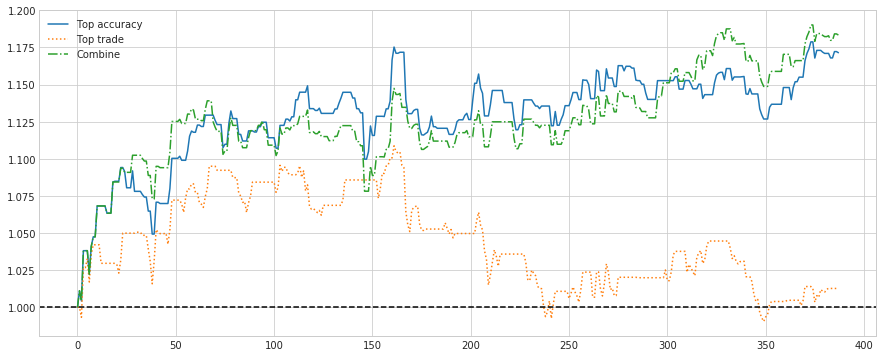
\includegraphics[width=\linewidth]{vs_macd_on_test}
\caption{Поведение торговых стратегий по сравнению с MACD на тестовой выборке}
\end{figure}

\begin{table}[h]
\centering
\begin{tabular}{| c | c | c |}
\hline
 & Среднее & Отклонение \\ \hline
Top trade & 1.04 & 0.030 \\ \hline
Top accuracy & 1.13 & 0.029 \\ \hline
Combine & 1.13 & 0.031 \\ \hline
\end{tabular}
\caption{Характеристики отношения стратегий к MACD на тестовой выборке}
\end{table}

Как можно увидеть, лидером является классификатор с максимальной точностью, но смешанная версия не сильно проседает по качеству.

Также была проверена гипотеза о зависимости предсказания от какого-либо периода (дни недели. начало месяца и проч.).
Стандартный для этого тест Льюнг-Бокса\cite{ljungbox} для индикаторов истинности предсказаний на тестовой выборке
показал $p$-значение 0.88, что позволяет уверенно заключить об отсутствии автокореляции.

\chapter{Итоги}

Таким образом, в данной работе была продемонстрирована возможность предсказания колебаний курса
валюты --- одного из финансовых показателей, основываясь исключительно на текство-новостной информации.
Более того, была также произведена демонстрация его применения для создания торговой стратегии,
которая выигрывает в сравнении с классической экономической стратегией MACD.

Несмотря на то, что выигрыш над MACD был достигнут, целью данной раоты в большей степени являлась иллюстрация
возможности такого предсказания, а не получение максимальной прибыли над MACD ценой узконаправленных эвристик,
из-за чего в продемонстрированном решении оставлено огромное поле для доработок.
На примере уже существующих работ в данной области можно порекомендовать смешение текстовых признаков и признаков,
описывающих численное поведение курса за небольшую историю; также нераскрытой остается возможность построения признакового
описания для каждой новости с последующим использованием их для представление дня.

\bibliography{literature}{}
\bibliographystyle{plain}

\end{document}